\tikzset{
  estilo nodos/.style={
      node distance=2.5cm,
      estado/.style={circle, draw, minimum size=1cm, inner sep=0pt},
      proba/.style={-latex, thin, bend left=20pt},
      every node/.style={font={\tiny}},
    },
  add flechas/.code={
      \draw[proba] (0) to node[above] {rec.} (1);
      \draw[proba] (1) to node[above] {rec.} (2);
      \draw[proba] (2) to node[above] {$\dots$} (dots.north west);
      \draw[proba] (dots.north east) to node[above] {$\dots$} (n-2);
      \draw[proba] (n-2) to node[above] {rec.} (n-1);
      \draw[proba] (n-1) to node[above] {rec.} (n);
    },
}
\begin{enunciado}{\ejercicio[CazadorDeFalsos]}

  \textit{CazadorDeFalsos}

  Se tiene una matriz booleana $A$ de $n \times n$ y una operación \textit{conjuncionSubmatriz} que toma $O(1)$ tiempo
  y que dados 4 enteros $i_0, i_1, j_0, j_1$ devuelve la conjunción de todos los elementos en la submatriz que toma las filas $i_0$
  hasta $i_1$ y las columnas $j_0$ hasta $j_1$. Formalmente:
  $$
    \textit{conjunciónSubmatriz}(i_0, i_1, j_0, j_1) =
    \conjuncion{i_0 \leq i \leq i_1 \\ j_0 \leq j \leq j_1}{}
    A[i,j]
  $$

  \begin{enumerate}[label=\arabic*.]
    \item Dar un algoritmo de complejidad temporal estrictamente menor que $O(n^2)$ que calcule la posición de algún
          \false, asumiendo que hay al menos uno. Calcular y justificar la complejidad del algoritmo.

    \item Modificar el algoritmo anterior para que cuente cuántos \false hay en la matriz. Asumiendo que hay
          a lo sumo 5 elementos \false en toda la matriz, calcular y justificar la complejidad del algoritmo.
          Esto se puede lograr con complejidad menor a $O(n^2)$.
  \end{enumerate}
\end{enunciado}

\begin{enumerate}[label=\arabic*.]
  \item
        \begin{itemize}
          \item Tengo una función mágica: \textit{\green{conjunciónSubmatriz}}. Agarra todos los elementos de la submatriz y si eso da \false,
                busco ahí adentro nuevamente para encontrar cuál elemento es el responsable de dar \false.

          \item Voy a estar dividiendo el input en 4 submatrices.

          \item Proceso solo la que me de \false, por lo tanto resuelvo solo 1 subproblema por llamado recursivo.

          \item Se parece a un \textit{binarySearch}.
        \end{itemize}

        \lstset{
          mathescape=true,
          emph={[1]funcion, return, ret, retorno},
          emph={[2]for,each, si, sino, if, else, true, false, not},
          emph={[3]cazadorDeFalsos, conjuncionSubmatriz},
          emphstyle={[1]\color{violet}\it},
          emphstyle={[2]\color{red}\it},
          emphstyle={[3]\color{OliveGreen}\it},
          morecomment={[l]{//}},
          commentstyle={\color{gray}\it\footnotesize}
        }
        \begin{tcolorbox}
          \begin{lstlisting}
funcion cazadorDeFalsos(f1, f2, c1, c2)
    si f1 = f2 $\land$ c1 = c2
        si A[f1,c1] = 0
            ret f1, c1
        sino
            ret "Esto no debería retornarse nunca. Hay al menos un 0 en A"

    fm $\ot$ (f1+f2)/2
    cm $\ot$ (c1+c2)/2

    si (not conjuncionSubmatriz(f1, fm, c1, cm))
        ret cazadorDeFalsos(f1, fm, c1, cm)
    si (not conjuncionSubmatriz(fm+1, f2, c1, cm))
        ret cazadorDeFalsos(fm+1, f2, c1, cm)
    si (not conjuncionSubmatriz(f1, fm, cm+1, c2))
        ret cazadorDeFalsos(f1, fm, cm+1, c2)
    si (not conjuncionSubmatriz(fm+1, f2, cm+1, c2))
        ret cazadorDeFalsos(fm+1, f2, cm+1, c2)

    ret "esto tampoco"
\end{lstlisting}
        \end{tcolorbox}

        Para calcular el \textit{running time} tengo:
        $$
          T(n^2) = T(n^2/4) + 1
        $$
        $$
          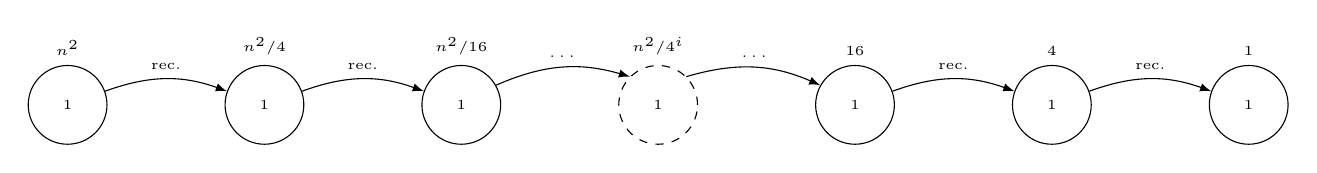
\begin{tikzpicture}[estilo nodos]
            \node[estado, label=above:{$n^2$}] (0) {$1$};
            \node[estado, right of=0, label=above:{$n^2/4$}] (1) {$1$};
            \node[estado, right of=1, label=above:{$n^2/16$}] (2) {$1$};
            \node[estado, right of=2, label={$n^2/4^i$}, dashed] (dots) {$1$};
            \node[estado, right of=dots, label=above:{$16$}] (n-2) {$1$};
            \node[estado, right of=n-2, label=above:{$4$}] (n-1) {$1$};
            \node[estado, right of=n-1, label=above:{$1$}] (n) {$1$};

            \draw[proba] (0) to node[above] {rec.} (1);
            \draw[proba] (1) to node[above] {rec.} (2);
            \draw[proba] (2) to node[above] {$\dots$} (dots.north west);
            \draw[proba] (dots.north east) to node[above] {$\dots$} (n-2);
            \draw[proba] (n-2) to node[above] {rec.} (n-1);
            \draw[proba] (n-1) to node[above] {rec.} (n);
          \end{tikzpicture}
        $$
        Como tengo una sola rama, la complejidad será contar la cantidad de iteraciones/nodos hasta llegar
        al caso base, dado que cada subproblema tiene un costo de $1$. La cantidad de niveles $k$ la calculo como:
        $$
          T((n^2/4^k)) = T(1)
          \sii
          (n^2/4^k) = 1
          \sii
          k = 2 \cdot \log_4(n)
          \Entonces{el \textit{running time}}
          \cajaResultado{
            T(n) \en \Theta(\log(n))
          }
        $$

  \item

        \begin{tcolorbox}
          \begin{lstlisting}
funcion cazadorDeFalsos(f1, f2, c1, c2)
    si f1 = f2 $\land$ c1 = c2
        si A[f1,c1] = 0
            ret 1
        sino 
            ret 0

    fm $\ot$ (f1+f2)/2
    cm $\ot$ (c1+c2)/2

    suma $\ot$ 0

    si (not conjuncionSubmatriz(f1, fm, c1, cm))
        suma = suma + cazadorDeFalsos(f1, fm, c1, cm)
    si (not conjuncionSubmatriz(fm+1, f2, c1, cm))
        suma = suma + cazadorDeFalsos(fm+1, f2, c1, cm)
    si (not conjuncionSubmatriz(f1, fm, cm+1, c2))
        suma = suma + cazadorDeFalsos(f1, fm, cm+1, c2)
    si (not conjuncionSubmatriz(fm+1, f2, cm+1, c2))
        suma = suma + cazadorDeFalsos(fm+1, f2, cm+1, c2)

    ret suma
\end{lstlisting}
        \end{tcolorbox}

        Para calcular el \textit{running time} tengo:
        $$
          T(n^2) =
          \llave{ccl}{
            1 & \text{si} & n = 1  \\
            4T(n^2/4) + 1 & \text{si} & n > 1
          }
        $$
        {\tiny
        $$
          \forestset{
          input/.style={label={[below left, xshift=-2pt, yshift=5pt]:{\tiny \red{ size \texttt{input}: $#1 \to$}}}},
          nivel/.style={label={[right, xshift=4pt, yshift=-3pt]:{\tiny \purple{$\ot$ \texttt{nivel}: $#1$}}}},
          binary tree/.style={
              for tree={
                  scale=0.4,
                  circle, draw, minimum size=0,
                  math content,
                  s sep=3pt, l sep=2pt,
                },
            }
          }
          \begin{forest}
            binary tree,
            [1, input={n^2}
                  [1,  input={n^2/4}
                      [\cdots,  input={n^2/4^i}
                          [1, input={1}]
                          [1]
                          [1]
                          [1]
                      ]
                      [\cdots
                        [1]
                        [1]
                        [1]
                        [1]
                      ]
                      [\cdots
                        [1]
                        [1]
                        [1]
                        [1]
                      ]
                  ]
                  [1
                      [\cdots
                        [1]
                        [1]
                        [1]
                        [1]
                      ]
                      [\cdots
                        [1]
                        [1]
                        [1]
                        [1]
                      ]
                      [\cdots
                        [1]
                        [1]
                        [1]
                        [1]
                      ]
                  ]
                  [1
                      [\cdots
                        [1]
                        [1]
                        [1]
                        [1]
                      ]
                      [\cdots
                        [1]
                        [1]
                        [1]
                        [1]
                      ]
                      [\cdots
                        [1]
                        [1]
                        [1]
                        [1]
                      ]
                  ]
                  [1
                      [\cdots
                        [1]
                        [1]
                        [1]
                        [1]
                      ]
                      [\cdots
                        [1]
                        [1]
                        [1]
                        [1]
                      ]
                      [\cdots
                        [1]
                        [1]
                        [1]
                        [1, nivel={\purple{2 \cdot \log_4(n)}}]
                      ]
                  ]
              ]
          \end{forest}
        $$
        }
        El árbol de recursión tiene 4 ramas en cada llamado. Dado que la función mágica $\textit{\green{conjunciónSubmatriz}}$ es O(1) contar
        la cantidad de nodos equivale al costo total:
        $$
          \sumatoria{i=0}{2\log_4(n)} 4^i = \frac{4^{2\log_4(n) + 1} - 1}{3} = \frac{4}{3}n^2 - \frac{1}{3} \en \Theta(n^2).
        $$

        ¿Esto me tendría que haber dado menos? Ignoré el dato de que hay \textit{a lo sumo 5 falsos}. El resultado obtenido es equivalente
        a haber recorrido \textit{absolutamente todos los elementos chequeando} si eran \true o \false. Lo cual
        tendría sentido si tuviese una cantidad arbitraría de 0's.

        Pero dado que \ul{como mucho tengo 5}, el ejercicio es equivalente al anterior, hay una cantidad constante de \textit{matricitas} que
        se van a detectar en las condiciones con \textit{\green{conjuncionSubmatriz}}. En el peor caso tendría:
        \begin{itemize}
          \item Un 0 en cada cuadrante, donde tendría 4 llamadas recursivas, $4/4$ (toda la matriz).
          \item En la segunda llamada ya búsqueda se reduce a solo $5/16$ partes de la matriz.
          \item Y en las sucesivas iteraciones la reducción: $5/4^3 \to 5/4^4 \to \cdots \to 5/4^k$ partes de la matriz, es exponencial.
        \end{itemize}
        El denominador de esas fracciones crece exponencialmente hasta llegar a $n^2$, es decir tiene $\approx 5\log_4(n)$ llamadas recursivas.
        Un árbol que tiene solo 5 ramas y $2\log(n)$ niveles. Algo así
        $$
          \sumatoria{i = 0}{5 \cdot \log_4(n)} 1  = 5 \log_4(n) \entonces
          \cajaResultado{
            T(n) \en \Theta(\log(n))
          }
        $$
\end{enumerate}

\fin
